
%导言区
\documentclass{article}%book,report,letter

\usepackage{ctex}
\usepackage{fontspec}
\usepackage{epsfig}
\usepackage{graphicx}
\usepackage{subfigure}
\usepackage{float}
\usepackage[namelimits]{amsmath} %数学公式
\usepackage{amssymb}             %数学公式
\usepackage{amsfonts}            %数学字体
\usepackage{mathrsfs}            %数学花体
%\usepackage{math}

%制作页眉页脚
\usepackage{fancyhdr}  
\pagestyle{fancy}  
\lhead{第二周作业}  
\chead{微分方程数值解法}  
\rhead{桑明达 15300180062}  
\lfoot{}  
\cfoot{\thepage}  
\rfoot{}  
\renewcommand{\headrulewidth}{0.4pt}  
\renewcommand{\footrulewidth}{0.4pt} 

%标题
\author{names}
\title{\heiti 微分方程数值解法\\ [2ex] \begin{large} 第二周作业 \end{large}}
\author{\kaishu 桑明达 15300180062}
\date{\today}

% 正文区
\begin{document}
\maketitle

%\newpage

\section{P24 2 比较不动点和Newton-Paphson迭代}

\begin{figure}[H]
	\begin{center}
		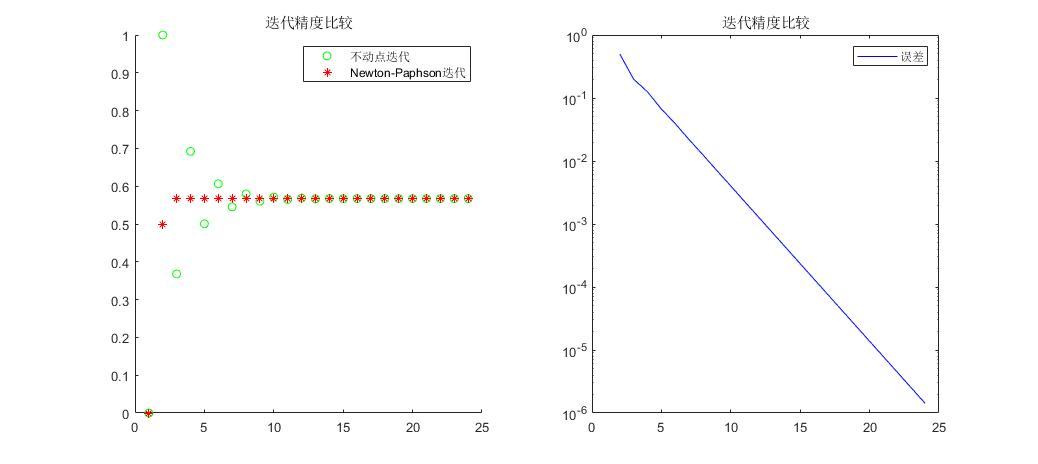
\includegraphics[width=1\linewidth]{week2.1.1.jpg}
		\caption{比较不动点迭代和Newton-Paphson迭代}
		\label{Fig:1}
	\end{center}
	\vspace{-0.5em}
\end{figure}

如图\ref{Fig:1},不动点迭代24次才能达到NP迭代4次的精度。

NP迭代相对于不动点迭代而言,方向性更准确,并且每一步的精确速率很高。

\newpage
\section{P34 1 证明范数等价关系}

\begin{enumerate}
	
	\item 左边的不等式
	\begin{displaymath} 
	\begin{aligned}	 
	\Vert{x} \Vert_p & = \sqrt[p]{\vert x \vert_1^p+\vert x \vert_2^p+\cdots+\vert x \vert_n^p} \\
	\Vert{x} \Vert_q & = \sqrt[q]{\vert x \vert_1^q+\vert x \vert_2^q+\cdots+\vert x \vert_n^q} \\
	\sum _{i=1}^n{\vert x \vert_i^q} & \leq \sum _{i=1}^n{{\vert x \vert_i^p}{\vert x \vert_i^{q-p}}}\\
	& = \sum _{i=1}^n{\vert x \vert_i^p}{(\vert x \vert_i^{p})^{\frac{q-p}{p}}} \\
	& \leq \sum _{i=1}^n{\vert x \vert_i^p}(\sum _{i=1}^n{\vert x \vert_i^{p})^{\frac{q-p}{p}}} \\
	& = (\sum _{i=1}^n{\vert x \vert_i^{p})^{1+\frac{q-p}{p}}} \\
	& = (\sum _{i=1}^n{\vert x \vert_i^{p})^{\frac{q}{p}}} \\
	\text{即证。}
	\end{aligned}
	\end{displaymath}
	
		\item 右边的不等式
	\begin{displaymath} 
	\begin{aligned}	
	\text{根据Jensen不等式} \\
	\sqrt[p]{\frac{\sum _{i=1}^n{\vert x \vert_i^p}}{n}} & \leq \sqrt[q]{\frac{\sum _{i=1}^n{\vert x \vert_i^q}}{n}}\\
		\text{即有} \\
	\sqrt[p]{\sum _{i=1}^n{\vert x \vert_i^p}} & \leq n ^{ \frac{1}{p} - \frac{1}{q} }\sqrt[q]{\sum _{i=1}^n{\vert x \vert_i^q}}\\
	\Vert{x} \Vert_p & \leq n ^{ \frac{1}{p} - \frac{1}{q} }\Vert{x} \Vert_q\\
	\text{即证}
	\end{aligned}
	\end{displaymath}

\end{enumerate}

\newpage
\section{P41 6 Runge现象}
分别用点数n=5,9,13时的等距节点插值公式,对Runge现象进行测试,如图\ref{Fig:2}

分别用点数n=5,9,13时的Chebyshev多项式极值点插值公式,对Runge现象进行测试,如图\ref{Fig:3}

可以看出,相对于等距节点插值公式,Chebyshev多项式极值点插值公式有更好的逼近性。\\

\begin{figure}[H]
	\begin{center}
		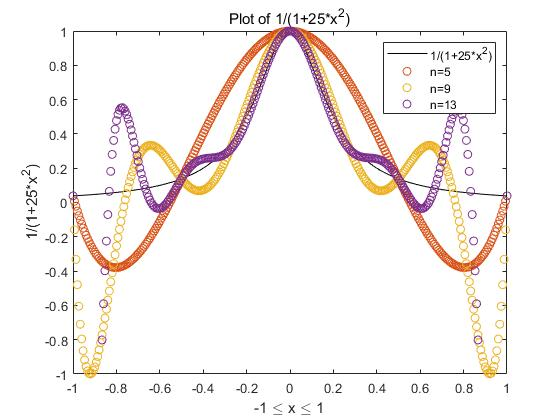
\includegraphics[width=1\linewidth]{week2.3.1.jpg}
		\caption{等距节点插值公式}
		\label{Fig:2}
	\end{center}
	\vspace{-0.5em}
\end{figure}

\begin{figure}[H]
	\begin{center}
		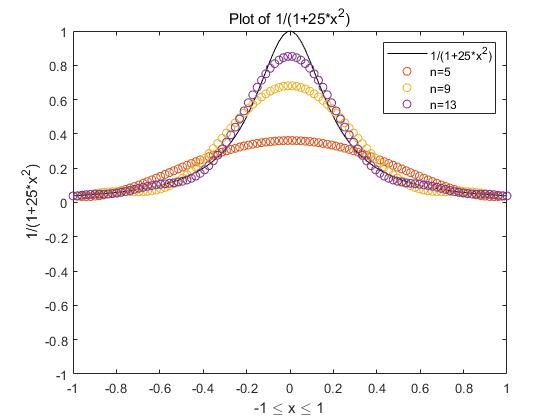
\includegraphics[width=1\linewidth]{week2.3.2.jpg}
		\caption{Chebyshev多项式极值点插值公式}
		\label{Fig:3}
	\end{center}
	\vspace{-0.5em}
\end{figure}

\end{document}